\NeedsTeXFormat{LaTeX2e}
\documentclass[twocolumn,letterpaper]{igs}
%\documentclass[review,letterpaper]{igs}

\usepackage{stfloats}
\usepackage{verbatim,xspace,amsmath,amssymb,bm}

\usepackage{tikz}
\usetikzlibrary{arrows}

\usepackage{igsnatbib}  % see igs2eguide.tex for example citation styles

\newcommand{\onecol}[1]{\includegraphics[width=86mm]{#1}}
\newcommand{\twocol}[1]{\includegraphics[width=178mm]{#1}}

% math macros
\newcommand\bb{\mathbf{b}}
\newcommand\bbf{\mathbf{f}}
\newcommand\bn{\mathbf{n}}
\newcommand\bq{\mathbf{q}}
\newcommand\bu{\mathbf{u}}
\newcommand\bv{\mathbf{v}}
\newcommand\by{\mathbf{y}}

\newcommand\bH{\mathbf{H}}
\newcommand\bQ{\mathbf{Q}}
\newcommand\bV{\mathbf{V}}
\newcommand\bW{\mathbf{W}}
\newcommand\bX{\mathbf{X}}

\newcommand\CC{\mathbb{C}}
\newcommand{\DDt}[1]{\ensuremath{\frac{d #1}{d t}}}
\newcommand{\ddt}[1]{\ensuremath{\frac{\partial #1}{\partial t}}}
\newcommand{\ddx}[1]{\ensuremath{\frac{\partial #1}{\partial x}}}
\newcommand{\ddy}[1]{\ensuremath{\frac{\partial #1}{\partial y}}}
\newcommand{\ddxp}[1]{\ensuremath{\frac{\partial #1}{\partial x'}}}
\newcommand{\ddz}[1]{\ensuremath{\frac{\partial #1}{\partial z}}}
\newcommand{\ddxx}[1]{\ensuremath{\frac{\partial^2 #1}{\partial x^2}}}
\newcommand{\ddyy}[1]{\ensuremath{\frac{\partial^2 #1}{\partial y^2}}}
\newcommand{\ddxy}[1]{\ensuremath{\frac{\partial^2 #1}{\partial x \partial y}}}
\newcommand{\ddzz}[1]{\ensuremath{\frac{\partial^2 #1}{\partial z^2}}}
\newcommand{\Div}{\nabla\cdot}
\newcommand\eps{\epsilon}
\newcommand{\grad}{\nabla}
\newcommand{\ihat}{\mathbf{i}}
\newcommand{\ip}[2]{\ensuremath{\left<#1,#2\right>}}
\newcommand{\jhat}{\mathbf{j}}
\newcommand{\khat}{\mathbf{k}}
\newcommand{\nhat}{\mathbf{n}}
\newcommand\lam{\lambda}
\newcommand\lap{\triangle}
\newcommand\RR{\mathbb{R}}
\newcommand\vf{\varphi}

\newcommand{\Mstar}{$\text{M}^{\bigstar}$\xspace}

\newcommand\alpharight{\alpha_{{}_{\blacktriangleright}}}
\newcommand\alphaup{\alpha_{{\!}_{\blacktriangle}}}

\newcommand{\dxtwo}{\tfrac{\Delta x}{2}}
\newcommand{\dytwo}{\tfrac{\Delta y}{2}}

\newcommand{\half}{\tfrac{1}{2}}


\begin{document}

\title[Stable FVE schemes for the shallow ice approximation]{Stable finite volume element schemes \\ for the shallow ice approximation}

\abstract{The isothermal, non-sliding shallow ice approximation, combined with mass conservation, is a model for ice sheet and glacier flow which should be used to determine the ice geometry as the solution of a free-boundary problem.  By solving the steady-state version of this problem, we demonstrate a fully-implicit scheme with no stability restrictions.  We first consider the \cite{Mahaffy1976} finite difference calculation of discrete flux, but interpreted as a ``finite volume element'' (FVE) scheme.  In this FVE context, everywhere-defined numerical fields and a finite volume integral form of the conservation statement are available, and on this basis we build an improved scheme which has both a better quadrature in the integral and upwinding on the part of the flux coming from the bed gradient.  By solving both the original and improved schemes in steady state by a parallel Newton scheme, respecting the constraint that thicknesses are nonnegative, we show that the improved scheme has superior accuracy to any published results for flat bed \citep{Bueler2003} and bedrock-step \citep{JaroschSchoofAnslow2013} exact solutions.  We then apply the improved scheme at 1km resolution to the compute the steady-state geometry of the Greenland ice sheet, using only bedrock elevation and present-day surface mass balance as input data, in a laptop-scale computation.}

\author{Ed Bueler}

\affiliation{Department of Mathematics and Statistics, and Geophysical Institute, University of Alaska Fairbanks, USA \\
E-mail: \emph{\texttt{elbueler\@@alaska.edu}}}

\maketitle

\sectionsize


\section*{Introduction}

The finite difference (FD) scheme introduced by \cite{Mahaffy1976} for modeling the Barnes Ice Cap was a first success in modeling ice sheet flow and geometry evolution in two horizontal dimensions.  The scheme solves the shallow ice approximation (SIA; Hutter, 1983)\nocite{Hutter1983} by computing the ice flux at staggered-grid points by particular choices for evaluating the ice surface slope and thickness.  An advantage of the scheme is its relatively-small stencil, which reduces memory usage in implicit implementations \citep{HindmarshPayne1996,Mahaffy1976} and interprocess communication in parallel implementations \citep{Bueleretal2007}.  Its stability and accuracy properties as an explicit scheme are relatively-well understood in flat-bed cases \citep{Bueleretal2005,HindmarshPayne1996}.  It can also be used as the deformational part of a membrane-stress-resolving hybrid stress balance solution method \citep{BuelerBrown2009}.

Existing numerical schemes for the SIA solve the time-dependent SIA with explicit, semi-implicit, or fully-implicit schemes with known or apparent stability restrictions \citep[among others]{Bueleretal2005,EgholmNielsen2010,HindmarshPayne1996,Huybrechtsetal1996,
JaroschSchoofAnslow2013}.  In these applications the SIA is solved with essentially \emph{ad hoc} treatment of the free margin of the ice sheet, for example using projection in explicit schemes to reset computed negative thicknesses back to zero \citep{Bueleretal2005,JaroschSchoofAnslow2013}.

\cite{JouvetBueler2012} construct the one exception to the above usage pattern.  They pose and numerically-solve the steady state SIA free-boundary problem as a variational inequality \citep{KinderlehrerStampacchia1980} which includes the nonnegative-ice-thickness constraint.  Here we follow \cite{JouvetBueler2012} in solving the steady state free-boundary problem, but we do it by re-interpreting the well-known Mahaffy method so that it becomes a highly-accurate and scalable scheme.  The new schemes are non-the-less easy to implement because Newton solvers modified to including the nonnegative-thickness constraint \citep{BensonMunson2006} are available within the open-source PETSc library \citep{Balayetal2014}.

In fact we show that the classical \cite{Mahaffy1976} FD scheme is simply a non-standard quadrature choice in a conforming finite element (FE) method.  The trial functions are piecewise-bilinear on a structured grid of rectangles---i.e.~$Q^1$ finite elements \citep{Elmanetal2005}.  The test functions are piecewise-constant with support on dual rectangular control volumes, so the scheme can be regarded as either a Petrov-Galerkin method \citep{Elmanetal2005} or as a ``finite volume element'' (FVE) method \citep{Cai1990,EwingLinLin2002}.  We adopt the FVE terminology because of the greater clarity which comes from regarding the mass conservation equation in classical flux-integral, i.e.~finite volume (FV; LeVeque, 2002),\nocite{LeVeque2002} form.

Based on this re-interpretation of the Mahaffy scheme we propose and test a ``\Mstar'' scheme which uses an obvious, and more accurate, quadrature choice when evaluating the finite volume flux integral.  The new scheme also uses first-order upwinding on the part of the flux that comes from the bedrock slope, but we see that the results are actually better than those from higher-resolution schemes when applied to a bedrock-step exact solution \citep{JaroschSchoofAnslow2013}.  Nonetheless the scheme is based on the same stencil, i.e.~uses only the same gridded values, as the classical Mahaffy scheme.  We also describe how to construct the improved scheme on unstructured finite element triangulations with dual control volumes, i.e.~Delaunay/Voronoi dual meshes \citep{EgholmNielsen2010,Ringleretal2013}.

\section*{Continuum model}

The time-dependent evolution equation for the ice thickness $H$ is a mass conservation equation,
\begin{equation}
\frac{\partial H}{\partial t} + \Div \bq = m,  \label{eq:siaevolution}
\end{equation}
where $\bq$ denotes the vertically-integrated flux (units $\text{m}^2/\text{s}$) and $m$ ($\text{m}/\text{s}$) is the surface mass balance, also called the accumulation/ablation function.  The divergence ``$\Div$'' is computed in horizontal $x,y$ directions only.

The SIA continuum model is the lubrication approximation \citep{Fowler1997} of the Stokes equations for slow-flowing ice, in non-sliding contact with the bed and with a freely-evolving upper surface.  We only consider the isothermal, Glen-power-law \citep{GreveBlatter2009} case.  Let $b$ be the bed and $s = H+b$ the ice surface elevation.  In the isothermal SIA the flux $\bq$ is given by
\begin{equation}
\bq = - \Gamma H^{n+2} |\grad s|^{n-1} \grad s  \label{eq:siaflux}
\end{equation}
where $\Gamma = 2 A (\rho g)^n / (n+2)$ is a positive constant derived from the Glen power $n$, the ice softness $A$, the ice density $\rho$, and gravity $g$ \citep{Bueleretal2005}.

The flux in \eqref{eq:siaflux} has multiple interpretations.  Equation \eqref{eq:siaevolution} is usually interpreted as nonlinear diffusion in which
\begin{equation}
\bq = - D \grad s \quad \text{and} \quad D =  \Gamma H^{n+2} |\grad s|^{n-1}. \label{eq:siafluxdiffusion}
\end{equation}
However, if the bed is not flat then $\grad s$ and $\grad H$ are different.  On the other hand one can compute a vertically-averaged velocity $\bV$, and suppose that the flux arises from the transport of the thickness by $\bV$, that is,
\begin{equation}
\bq = \bV H \quad \text{where} \quad \bV = - \Gamma H^{n+1} |\grad s|^{n-1} \grad s. \label{eq:siafluxvelocity}
\end{equation}
In this case \eqref{eq:siaevolution} is, apparently, a hyperbolic conservation equation, but this appearance is superficial because the velocity depends in part on the gradient of the transported quantity.

The former diffusion interpretation \eqref{eq:siafluxdiffusion} is more appropriate in the flat-bed case $b=0$ because in that case \eqref{eq:siaevolution} can be transformed to a $p$-Laplacian diffusion equation \citep{Calvoetal2002}.  In general, however, the diffusion-equation interpretation of \eqref{eq:siaevolution} is obscured by the bed gradient $\grad b$ which is in formula \eqref{eq:siafluxdiffusion} for $D$.  This bed gradient is a barrier to theoretical progress on proving the existence and uniqueness of solutions \citep{JouvetBueler2012} and it generates conservation errors at the ice margin in numerical schemes \citep{JaroschSchoofAnslow2013}.

Later in this paper we will settle on a modification of the flux form suggested by \cite{JaroschSchoofAnslow2013}, namely
\begin{equation}
\bq = - D \grad H + \bW H^{n+2},\label{eq:fluxform}
\end{equation}
where $D$ is the same as in \eqref{eq:siafluxdiffusion} and
\begin{equation}
\bW = - \Gamma |\grad s|^{n-1} \grad b.  \label{eq:siaWdefine}
\end{equation}
The vector field $\bW$ can be thought of as a ``velocity'' which transports $H^{n+2}$; compare ``$\boldsymbol{\omega}$'' in equation (19) in \citep{JaroschSchoofAnslow2013}.  Note that $\bW=0$ in the case of flat beds.  The advantage of form \eqref{eq:fluxform} in numerical schemes, over either \eqref{eq:siafluxdiffusion} or \eqref{eq:siafluxvelocity}, is that we can apply a non-oscillatory transport scheme to the ``$\bW H^{n+2}$'' term while preserving accuracy by applying a centered scheme to the diffusive term ``$-D \grad H$''.

In this paper we solve only the steady-state form of \eqref{eq:siaevolution},
\begin{equation}
\Div \bq = m.  \label{eq:siasteady}
\end{equation}
Though this equation is simpler than \eqref{eq:siaevolution}, it is more difficult to solve in the sense that the location where the boundary conditions should be applied is unknown \citep{JaroschSchoofAnslow2013,JouvetBueler2012}, that is, it is a free-boundary problem.  The domain where \eqref{eq:siasteady} applies, and the location of the boundary where $\bq=0$, cannot be treated as a small modification of a known boundary, the standard approach of time-stepping schemes \citep{Bueleretal2005,Huybrechtsetal1996}.

Numerical solutions of the steady problem \eqref{eq:siasteady} are closely-related to fully-implicit  solutions of \eqref{eq:siaevolution}.  Suppose we discretize \eqref{eq:siaevolution} only in time (``semi-discretized'') by the backward Euler method.  Denoting the approximate thickness function at time $t_l$ by $H_l$, we have a problem essentially the same as \eqref{eq:siasteady} at each time-step $\Delta t> 0$:
\begin{equation}
\Delta t\,\Div \bq_l + H_l = \Delta t\,m + H_{l-1}.  \label{eq:siaBE}
\end{equation}
Here the unknown flux $\bq_l$ depends on the thickness solution $H_l$ via a flux formula (e.g.~\eqref{eq:fluxform}).  If the surface mass balance $m$ is independent of surface elevation then the right side of \eqref{eq:siaBE} is known, just as in \eqref{eq:siasteady}.  Solving \eqref{eq:siaBE} can be done by exactly the same kind of spatial discretization and constrained-Newton method as we apply to \eqref{eq:siasteady}.  Both equations should be solved as free boundary problems of ``elliptic'' type \citep{JouvetBueler2012}.

The problem we solve consists of equations \eqref{eq:fluxform} and \eqref{eq:siasteady}, where $D$, $\bW$ are defined in \eqref{eq:siafluxdiffusion}, \eqref{eq:siaWdefine} respectively.  The input data to this problem consists of the bed elevation $b(x,y)$ and the (steady) surface mass balance $m(x,y)$ defined on some larger domain $\Omega$.  The solution is the nonnegative thickness function $H(x,y)$, and corresponding surface elevation $s(x,y)$.

If $m$ is sufficiently-negative near the boundary of $\Omega$ then $H$ reaches zero inside the domain at a free boundary \citep{JouvetBueler2012}.  This free boundary, at which both $H\to 0$ and $\bq \to 0$, also has degenerate diffusivity $D \to 0$.  Solving equation \eqref{eq:siasteady}, or each time-step equation \eqref{eq:siaBE}, as such a free-boundary problem, without a boundary flux applied along any part of the boundary of $\Omega$, is usually called a ``whole'' ice sheet model.  We restrict our attention to such whole ice sheet models.


\section{Classical Mahaffy scheme}   \label{sec:mahaffyfd}

Consider the rectangular structured FD grid in Figure \ref{fig:fdfemgrids}a with spacing $\Delta x,\Delta y$.  The Mahaffy scheme calculates $\bq$ at the staggered grid points marked by a triangles in the Figure; see equations (19) and (20) in \cite{Mahaffy1976}.  Specifically, at $(x_{j+\half},y_k)$ the scheme computes the $x$-component of the flux by
\begin{equation}
q^x_{j+\half,k} = - \Gamma (H_{j+\half,k})^{\,n+2} \alpharight^{\,n-1} \frac{s_{j+1,k} - s_{j,k}}{\Delta x}  \label{eq:mahaffyqx}
\end{equation}
where $s_{j,k} = H_{j,k} + b_{j,k}$.  In \eqref{eq:mahaffyqx} the staggered-grid value of the thickness is simply the average
\begin{equation}
  H_{j+\half,k} = \frac{H_{j,k} + H_{j+1,k}}{2},  \label{eq:mahaffyHav}
\end{equation}
and the quantity ``$\alpharight$\!'' is an estimate of $|\grad s|$:
\begin{align}
\alpharight^{\,2} &= \left(\frac{s_{j+1,k} - s_{j,k}}{\Delta x}\right)^2  \label{eq:mahaffyalphax} \\
  &\quad + \left(\frac{s_{j,k+1} + s_{j+1,k+1} - s_{j,k-1} - s_{j+1,k-1}}{4 \Delta y}\right)^2. \notag
\end{align}
The formula for the flux $q^y_{j,k+\half}$ at staggered location $(x_j,y_{k+\half})$, which uses thickness average $H_{j,k+\half}$ and slope estimate $\alphaup$, follows by swapping the roles of $j$ and $k$, and $\Delta x$ and $\Delta y$, in the above equations.

\begin{figure}[ht]
\begin{center}
\begin{tikzpicture}[scale=0.75]
  %uncomment to see grid on which it was generated:
  %\draw[dotted,step=1.0,black,very thin] (0,0) grid (6,4);

  % faint grid
  \draw[gray, dashed] (-0.75,0) -- (6.75,0);
  \draw[gray, dashed] (-0.75,2) -- (6.75,2);
  \draw[gray, dashed] (-0.75,4) -- (6.75,4);
  \draw[gray, dashed] (0,-0.5) -- (0,4.5);
  \draw[gray, dashed] (3,-0.5) -- (3,4.5);
  \draw[gray, dashed] (6,-0.5) -- (6,4.5);

  % regular FD points
  \filldraw (0,0) circle (2.5pt);
  \filldraw (3,0) circle (2.5pt);
  \filldraw (6,0) circle (2.5pt);
  \filldraw (0,2) circle (2.5pt);
  \filldraw (3,2) circle (2.5pt);
  \filldraw (6,2) circle (2.5pt);
  \filldraw (0,4) circle (2.5pt);
  \filldraw (3,4) circle (2.5pt);
  \filldraw (6,4) circle (2.5pt);

  % staggered FD points
  \def\dx{0.12};
  \filldraw (1.5-\dx,2+\dx) -- (1.5+\dx,2) -- (1.5-\dx,2-\dx) -- cycle;
  \filldraw (4.5-\dx,2+\dx) -- (4.5+\dx,2) -- (4.5-\dx,2-\dx) -- cycle;
  \filldraw (3-\dx,1-\dx) -- (3,1+\dx) -- (3+\dx,1-\dx) -- cycle;
  \filldraw (3-\dx,3-\dx) -- (3,3+\dx) -- (3+\dx,3-\dx) -- cycle;

  % dimensions \Delta x, \Delta y
  \draw[latex-latex] (3.2,4.5) -- (5.8,4.5);
  \draw (4.5,5.0) node {$\Delta x$};
  \draw[latex-latex] (6.5,2.2) -- (6.5,3.8);
  \draw (7.0,3) node {$\Delta y$};

  % label center point and dims
  \draw (3,-1.0) node {$x_j$};
  \draw (-1.25,2) node {$y_k$};

  % label as "a"
  \draw (-1.5,5.5) node {{\large a.}};
\end{tikzpicture}
 \quad 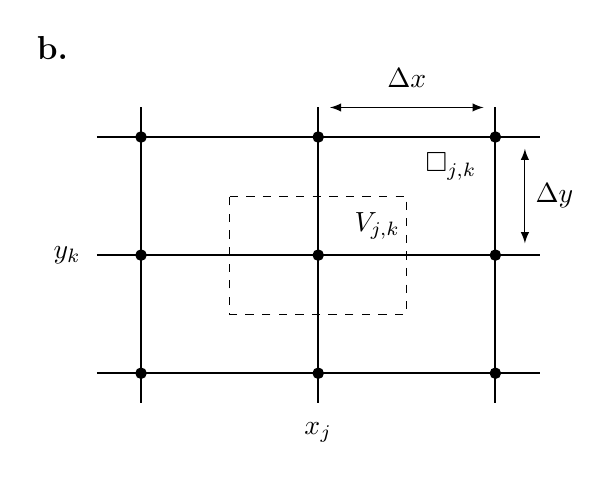
\begin{tikzpicture}[scale=0.75]
  %uncomment to see grid on which it was generated:
  %\draw[dotted,step=1.0,black,very thin] (0,0) grid (6,4);

  % strong grid around elements
  \draw[thick] (-0.75,0) -- (6.75,0);
  \draw[thick] (-0.75,2) -- (6.75,2);
  \draw[thick] (-0.75,4) -- (6.75,4);
  \draw[thick] (0,-0.5) -- (0,4.5);
  \draw[thick] (3,-0.5) -- (3,4.5);
  \draw[thick] (6,-0.5) -- (6,4.5);

  % nodes
  \filldraw (0,0) circle (2.5pt);
  \filldraw (3,0) circle (2.5pt);
  \filldraw (6,0) circle (2.5pt);
  \filldraw (0,2) circle (2.5pt);
  \filldraw (3,2) circle (2.5pt);
  \filldraw (6,2) circle (2.5pt);
  \filldraw (0,4) circle (2.5pt);
  \filldraw (3,4) circle (2.5pt);
  \filldraw (6,4) circle (2.5pt);

  % outline control volume
  \draw[dashed] (1.5,3) -- (4.5,3) -- (4.5,1) -- (1.5,1) -- cycle;

  % label element and control volume
  \draw (5.25,3.5) node {$\square_{j,k}$};
  \draw (4,2.5) node {$V_{j,k}$};

  % dimensions \Delta x, \Delta y
  \draw[latex-latex] (3.2,4.5) -- (5.8,4.5);
  \draw (4.5,5.0) node {$\Delta x$};
  \draw[latex-latex] (6.5,2.2) -- (6.5,3.8);
  \draw (7.0,3) node {$\Delta y$};

  % label center point and dims
  \draw (3,-1.0) node {$x_j$};
  \draw (-1.25,2) node {$y_k$};

  % label as "b"
  \tikzstyle{fontbf} = [font=\bf]
  \draw (-1.5,5.5) node[fontbf] {{\large b.}};
\end{tikzpicture}

\end{center}
\caption{\textbf{a.}~A structured FD grid with regular points (dots) and staggered points (triangles).  \textbf{b.}~The same grid as an FVE grid with rectangular elements $\square_{j,k}$ (solid), nodes (dots), and a dual rectangular control volume $V_{j,k}$ (dashed).}
\label{fig:fdfemgrids}
\end{figure}

Slope approximation \eqref{eq:mahaffyalphax}, and its modifications for the other staggered grid points, is the least-obvious aspect of the Mahaffy scheme.  However, \cite{Mahaffy1976} discretizes the SIA equation \eqref{eq:siasteady} by straightforward centered-difference formulas \citep{MortonMayers2005}:
\begin{equation}
\frac{q^x_{j+1/2,k} - q^x_{j-1/2,k}}{\Delta x} + \frac{q^y_{j,k+1/2}- q^y_{j,k-1/2}}{\Delta y} = m_{j,k}.  \label{eq:siasteadyfd}
\end{equation}

Equation \eqref{eq:siasteadyfd} is one equation in an algebraic system which determines all values $H_{j,k}$ simultaneously.  Equation \eqref{eq:siasteadyfd}, centered at $(x_j,y_k)$, involves all nine unknown values of $H$ at the regular grid points in Figure \ref{fig:fdfemgrids}a.  We call this pattern of dependence the ``stencil'' of the scheme \citep{MortonMayers2005}.


\section{FVE\, Interpretation} \label{sec:fveinterpretation}

The above description of the Mahaffy FD method is familiar to numerical ice sheet modelers, but we now re-derive the scheme from an FE \emph{and} FV perspective.  Our re-interpretation uses the same structured grid, but the regular grid points $(x_j,y_k)$ are now nodes (degrees of freedom) for a continuous space of trial functions.  The same nodes are also used as centered degrees of freedom for (discontinuous) piecewise-constant test functions.  These test functions are discontinuous at the FD method's staggered grid points in particular (Figure \ref{fig:fdfemgrids}).  The method is a ``finite volume element'' (FVE) method in which exact discrete conservation, and the construction of upwind-type flux components, will follow in the standard FV understanding.  The FE character remains in that we use values of the interpolating trial function, from the interior of the element, in evaluating the finite volume integral.

To re-derive the Mahaffy scheme we suppose \eqref{eq:siasteady} holds and we apply the divergence theorem to a subregion $V$ of $\Omega$:
\begin{equation}
  \int_{\partial V} \bq \cdot \bn\,ds = \int_V m\, dx\,dy. \label{eq:siaasconservation}
\end{equation}
Here $\partial V$ denotes the boundary of $V$, $\bn$ is the outward normal unit vector, and $ds$ the length element on the closed curve $\partial V$.  Equation \eqref{eq:siaasconservation} is simply the integral form of \eqref{eq:siasteady}.

An FVE method supposes that the approximation $H^h$ of the thickness solution lies in a finite-dimensional space of continuous functions which are differentiable almost everywhere.  These functions are sufficiently well-behaved so that the approximate flux $\bq^h$ is defined almost everywhere and can be integrated along $\partial V$ in \eqref{eq:siaasconservation}.  In the method, integral equation \eqref{eq:siaasconservation} is required to hold for a finite set of volumes $V$ which together tile $\Omega$.  This generates a finite system of nonlinear algebraic equations which can be solved by Newton's method (see Examples section).  This derivation of the algebraic system uses \eqref{eq:siaasconservation} the same way an FV method would solve differential equation \eqref{eq:siasteady}.

Again consider the structured grid of rectangular elements shown in Figure \ref{fig:fdfemgrids}b.  Denote the element with lower-left corner at $(x_j,y_k)$ by $\square_{j,k}$.  These rectangles are $Q^1$ finite elements \citep{Elmanetal2005} when associated with bilinear functions.  A basis for such functions on $\square_{j,k}$ is a set of four functions
\begin{equation}
\chi_l\left(\frac{x-x_j}{\Delta x},\frac{y-y_k}{\Delta y}\right)  \label{eq:elementbasis}
\end{equation}
where
\begin{align*}
\chi_1(\xi,\nu) &= \left(1-\xi\right) \left(1-\nu\right), & \chi_2(\xi,\nu) &= \xi \left(1-\nu\right), \\
\chi_3(\xi,\nu) &= \left(1-\xi\right) \nu, & \chi_4(\xi,\nu) &= \xi \nu.
\end{align*}
Now let
\begin{equation}
S_h = \{u \text{ is bilinear on each $\square_{j,k}$}\}
\end{equation}
be the trial space of continuous functions.  Functions in $S_h$ have a gradient which is defined almost everywhere, but the gradient is discontinuous along the element edges (solid lines in Figure \ref{fig:fdfemgrids}b).

Let $V_{j,k}$ be the control volume with center at $(x_j,y_j)$ (Figure \ref{fig:fdfemgrids}b).  Let
\begin{equation}
S_h^* = \{u \text{ is constant on each $V_{j,k}$}\}
\end{equation}
be the test space of functions which are piecewise constant and discontinuous along the control volume edges (dashed lines in Figure \ref{fig:fdfemgrids}b).

\begin{figure}[ht]
\begin{center}
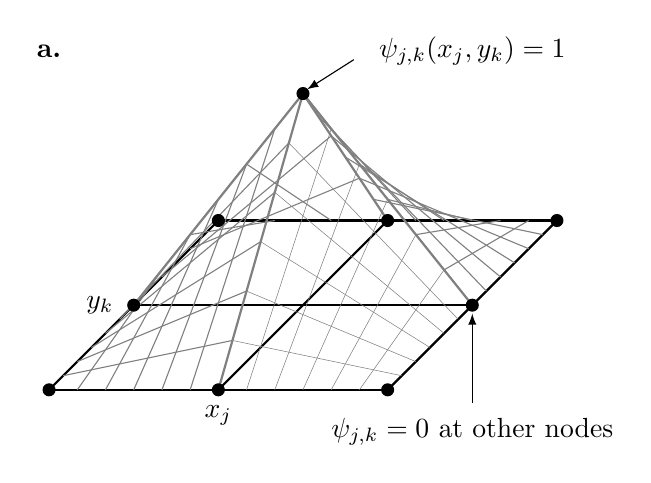
\begin{tikzpicture}[scale=8.6cm/16.0cm]
% min x = 0, max x = 12  so  width = 12 cm, but we pad
% 8.6cm is one-column width for J Glaciol
%\begin{tikzpicture}[scale=0.5]

  % strong grid around elements
  \draw[thick] (0,0) -- (8,0);
  \draw[thick] (2,2) -- (10,2);
  \draw[thick] (4,4) -- (12,4);
  \draw[thick] (0,0) -- (4,4);
  \draw[thick] (4,0) -- (8,4);
  \draw[thick] (8,0) -- (12,4);

  \def\ytop{7};

  % tent lines
  \draw[gray,thick] (6,\ytop) -- (4,0);
  \draw[gray,thick] (6,\ytop) -- (2,2);
  \draw[gray,thick] (6,\ytop) -- (10,2);
  \draw[gray,thick] (6,\ytop) -- (8,4);

  \def\dx{(10.0-6.0)/6};
  \def\dy{(2.0-\ytop)/6};
  \foreach \jj in {1,...,5}
  {
       \draw[gray,very thin] ({6+\jj*\dx},{\ytop+\jj*\dy}) -- ({4+(4/6)*\jj},0.0);
  }

  \def\dx{(4.0-6.0)/6};
  \def\dy{(0.0-\ytop)/6};
  \foreach \jj in {1,...,5}
  {
       \draw[gray,very thin] ({6+\jj*\dx},{\ytop+\jj*\dy}) -- ({10-(2/6)*\jj},{2-(2/6)*\jj});
  }

  \def\dx{(2.0-6.0)/6};
  \def\dy{(2.0-\ytop)/6};
  \foreach \jj in {1,...,5}
  {
       \draw[gray,thin] ({6+\jj*\dx},{\ytop+\jj*\dy}) -- ({4-(4/6)*\jj},0.0);
  }

  \def\dx{(4.0-6.0)/6};
  \def\dy{(0.0-\ytop)/6};
  \foreach \jj in {1,...,5}
  {
       \draw[gray,thin] ({6+\jj*\dx},{\ytop+\jj*\dy}) -- ({2-(2/6)*\jj},{2-(2/6)*\jj});
  }

  \def\dx{(10.0-6.0)/6};
  \def\dy{(2.0-\ytop)/6};
  \foreach \jj in {1,...,5}
  {
       \draw[gray,thin] ({6+\jj*\dx},{\ytop+\jj*\dy}) -- ({8+(4/6)*\jj},4.0);
  }

  \def\dx{(8.0-6.0)/6};
  \def\dy{(4.0-\ytop)/6};
  \foreach \jj in {1,...,5}
  {
       \draw[gray,thin] ({6+\jj*\dx},{\ytop+\jj*\dy}) -- ({10+(2/6)*\jj},{2+(2/6)*\jj});
  }

  \def\dx{(2.0-6.0)/3};
  \def\dy{(2.0-\ytop)/3};
  \foreach \jj in {1,...,2}  % reduce clutter
  {
       \draw[gray,thin] ({6+\jj*\dx},{\ytop+\jj*\dy}) -- ({8-(4/3)*\jj},4.0);
  }

  \def\dx{(8.0-6.0)/3};
  \def\dy{(4.0-\ytop)/3};
  \foreach \jj in {1,...,2}
  {
       \draw[gray,thin] ({6+\jj*\dx},{\ytop+\jj*\dy}) -- ({2+(2/3)*\jj},{2+(2/3)*\jj});
  }

  % nodes in base plane
  \filldraw (0,0) circle (4pt);
  \filldraw (4,0) circle (4pt);
  \filldraw (8,0) circle (4pt);
  \filldraw (2,2) circle (4pt);
  %\filldraw (6,2) circle (4pt);   % (x_j,y_k) is at (6,2)
  \filldraw (10,2) circle (4pt);
  \filldraw (4,4) circle (4pt);
  \filldraw (8,4) circle (4pt);
  \filldraw (12,4) circle (4pt);

  % node at tent top
  \filldraw (6,\ytop) circle (4pt);

  % annotate
  \draw (10,\ytop+1.0) node {$\psi_{j,k}(x_j,y_k)=1$};
  \draw[-latex] (7.2,\ytop+0.8) -- (6.1,\ytop+0.1);
  \draw (10,-1.0) node {$\psi_{j,k}=0$ at other nodes};
  \draw[-latex] (10,-0.3) -- (10,1.8);

  % label center point
  \draw (4,-0.6) node {$x_j$};
  \draw (1.2,2) node {$y_k$};

  % label as "a"
  \tikzstyle{fontbf} = [font=\bf]
  \draw (0,8) node[fontbf] {a.};

\end{tikzpicture}
 \quad 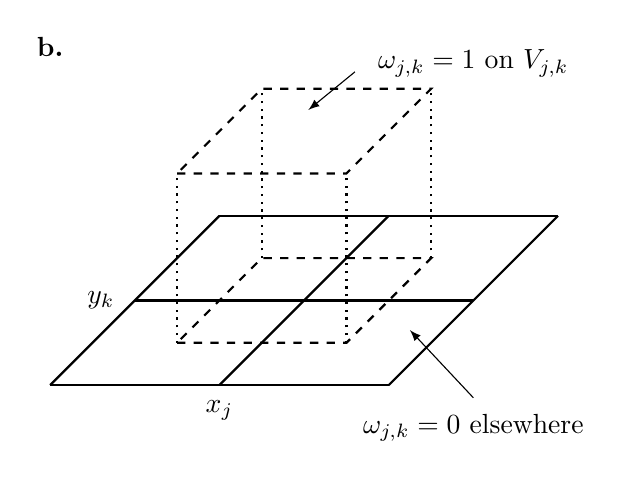
\begin{tikzpicture}[scale=8.6cm/16.0cm]
% min x = 0, max x = 12  so  width = 12 cm, but we pad
% 8.6cm is one-column width for J Glaciol
%\begin{tikzpicture}[scale=0.5]

  % strong grid around elements
  \draw[thick] (0,0) -- (8,0);
  \draw[thick] (2,2) -- (10,2);
  \draw[thick] (4,4) -- (12,4);
  \draw[thick] (0,0) -- (4,4);
  \draw[thick] (4,0) -- (8,4);
  \draw[thick] (8,0) -- (12,4);

  % dashed grid around control volume in base plane
  \draw[thick] (0,0) -- (8,0);

  % label element and control volume
  \def\lift{4};
  \draw[dashed, thick] (3,1) -- (7,1) -- (9,3) -- (5,3) -- cycle;
  \draw[dashed, thick] (3,1+\lift) -- (7,1+\lift) -- (9,3+\lift) -- (5,3+\lift) -- cycle;
  \draw[dotted, thick] (3,1) -- (3,1+\lift);
  \draw[dotted, thick] (7,1) -- (7,1+\lift);
  \draw[dotted, thick] (9,3) -- (9,3+\lift);
  \draw[dotted, thick] (5,3) -- (5,3+\lift);

  % annotate
  \draw (10,\lift+3.6) node {$\omega_{j,k}=1$ on $V_{j,k}$};
  \draw[-latex] (7.2,\lift+3.4) -- (6.1,\lift+2.5);
  \draw (10,-1.0) node {$\omega_{j,k}=0$ elsewhere};
  \draw[-latex] (10,-0.3) -- (8.5,1.3);

  % label center point
  \draw (4,-0.6) node {$x_j$};
  \draw (1.2,2) node {$y_k$};

  % label as "b"
  \tikzstyle{fontbf} = [font=\bf]
  \draw (0,8) node[fontbf] {b.};

\end{tikzpicture}

\end{center}
\caption{\textbf{a.}~A continuous ``hat'' basis function $\psi_{j,k}(x,y)$ in the trial space $S_h$.  \textbf{b.}~A discontinuous, piecewise-constant basis function $\omega_{j,k}(x,y)$ in the test space $S_h^*$.}
\label{fig:fembases}
\end{figure}

Bases of $S_h$ and $S_h^*$ are formed by those functions which take value one at a single node, and zero at all other nodes.  By definition, $\psi_{j,k}(x,y)$ is the unique function in $S_h$ so that $\psi_{j,k}(x_r,y_s) = \delta_{jr} \delta_{ks}$, while $\omega_{j,k}(x,y)$ is the unique function in $S_h^*$ so that $\omega_{j,k}(x_r,y_s) = \delta_{jr} \delta_{ks}$; see Figure \ref{fig:fembases}.  We will use a periodic grid with $N_x$ rectangles in the $x$-direction and $N_y$ in the $y$ direction, so there are $N_xN_y$ distinct nodes and $\dim S_h = \dim S_h^* = N_x N_y$.  


We seek an approximate solution $H^h$ from $S_h$.  Let $b^h$ be the piecewise-bilinear interpolant of the bed elevation $b$, and let $s^h=H^h+b^h$, so both are in $S_h$.  We denote by $\bq^h$ the flux computed from formula \eqref{eq:siaflux} using $H^h$ and $b^h$, so $\bq^h$ is well-defined on the interior of each element.  We require \eqref{eq:siaasconservation} to hold for this $\bq^h$ and all volumes $V_{j,k}$, but this is equivalent to multiplying \eqref{eq:siasteady} by any $\omega_{j,k}$ and then integrating.  We use midpoint quadrature on the right-hand integral in \eqref{eq:siaasconservation}.  Thus we seek $H^h$ in $S_h$ satisfying
\begin{equation}
  \int_{\partial V_{j,k}} \bq^h \cdot \bn\,ds = m_{j,k}\, \Delta x \Delta y, \label{eq:siafve}
\end{equation}
for all $j,k$.  This gives a finite algebraic system once we choose a quadrature rule on the left.

We decompose the integral in \eqref{eq:siafve} into the four edges which form $\partial V_{j,k}$.  Let
\begin{equation}
x_j^\pm = x_j \pm \dxtwo, \qquad y_k^\pm = y_k \pm \dytwo, \label{eq:definexypm}
\end{equation}
and denote components $\bq^h = \ip{q^x}{q^y}$, so that
\begin{align}
\int_{\partial V_{j,k}} \bq^h \cdot \bn\,ds &= \int_{y_k^-}^{y_k^+} q^x(x_j^+,y)\,dy \label{eq:fluxintdecomp} \\
&\quad + \int_{x_j^-}^{x_j^+} q^y(x,y_k^+)\,dx \notag \\
&\quad - \int_{y_k^-}^{y_k^+} q^x(x_j^-,y)\,dy \notag \\
&\quad - \int_{x_j^-}^{x_j^+} q^y(x,y_k^-)\,dx. \notag
\end{align}

Note $\bq^h$ is a well-defined, bounded function which is continuous on each element $\square_{j,k}$.  However, it is discontinuous across element boundaries.  For example, in the first integral on the right in \eqref{eq:fluxintdecomp} the integrand $f(y) = q^x(x_j^+,y)$ has a jump discontinuity at the midpoint $y=y_k$ of the interval of integration $y_k^- \le y \le y_k^+$ because $s^h_y$ is discontinuous there.  On the other hand, formula \eqref{eq:mahaffyqx} in the Mahaffy FD scheme computes the normal component of $\bq^h$ at the center of the right edge of the control volume shown in Figure \ref{fig:fdfemgrids}b, which is the just-described midpoint in the first integral in \eqref{eq:fluxintdecomp}.

In fact the Mahaffy scheme computes each integral in \eqref{eq:fluxintdecomp} by the midpoint method, but by \emph{averaging the discontinuous component of the surface gradient across its jump discontinuity}.  Thus Mahaffy does not use a true quadrature, because the integrand $\bq^h\cdot \bn$ does not have a value at the quadrature point (i.e.~the midpoint).

To turn this idea into FVE formulas, observe that the thickness $H^h$ and the $x$-derivative $s^h_x$ are continuous along the edge between elements $\square_{j,k}$ and $\square_{j,k-1}$.  Indeed, using the element basis \eqref{eq:elementbasis} the surface gradient on $\square_{j,k}$ has components
\begin{align}
s^h_x(x,y) &= \frac{s_{j+1,k}-s_{j,k}}{\Delta x} \left(1-\frac{y-y_k}{\Delta y}\right)  \label{eq:grads} \\
   &\quad + \frac{s_{j+1,k+1}-s_{j,k+1}}{\Delta x} \left(\frac{y-y_k}{\Delta y}\right), \notag \\
s^h_y(x,y) &= \frac{s_{j,k+1}-s_{j,k}}{\Delta y} \left(1-\frac{x-x_j}{\Delta x}\right) \notag \\
   &\quad + \frac{s_{j+1,k+1}-s_{j+1,k}}{\Delta y} \left(\frac{x-x_j}{\Delta x}\right). \notag
\end{align}
The same functions on $\square_{j,k-1}$ can be calculated by shifting the index $k$ to $k-1$.  Thus the continuous function $s^h_x(x,y)$ has value
\begin{equation}
s^h_x(x_j^+,y_k) = \frac{s_{j+1,k}-s_{j,k}}{\Delta x} \label{eq:femsxstag}
\end{equation}
at the midpoint in the first integral in \eqref{eq:fluxintdecomp}.  Similarly, writing-out $H^h(x,y)$ using the element basis \eqref{eq:elementbasis} gives
\begin{equation}
H^h(x_j^+,y_k) = \frac{H_{j,k}+H_{j+1,k}}{2} \label{eq:femHstag}
\end{equation}
at the midpoint.

However, the $y$-derivative has different values above (i.e.~on $\square_{j,k}$) and below (on $\square_{j,k-1}$) the element boundary at $y = y_k$; the limits are:
\begin{align}
s^h_y(x_j^+,y_k+0) = \frac{s_{j,k+1}-s_{j,k} + s_{j+1,k+1}-s_{j+1,k}}{2\Delta y}, \\
s^h_y(x_j^+,y_k-0) = \frac{s_{j,k}-s_{j,k-1} + s_{j+1,k}-s_{j+1,k-1}}{2\Delta y}. \notag
\end{align}
The average of these values is not a value of $s_y^h$---thus the hat notation---but a re-construction thereof:
\begin{equation}
\widehat{s^h_y}(x_j^+,y_k) = \frac{s_{j,k+1} + s_{j+1,k+1} - s_{j,k-1} - s_{j+1,k-1}}{4\Delta y}. \label{eq:femsystagcrime}
\end{equation}
Formula \eqref{eq:femsystagcrime} is exactly the estimate of $\partial s/\partial y$ which appears in FD formula \eqref{eq:mahaffyalphax}.

In our FVE interpretation, the Mahaffy scheme uses \eqref{eq:femsxstag}, \eqref{eq:femHstag}, and \eqref{eq:femsystagcrime} in the midpoint rule:
\begin{align}
&\int_{y_k^-}^{y_k^+} q^x(x_j^+,y)\,dy  \label{eq:femmahaffyfirstint} \\
  &\quad\approx - \Delta y\, \Gamma H^h(x_j^+,y_k)^{n+2} \,\alpharight^{\,(n-1)/2} s^h_x(x_j^+,y_k). \notag 
\end{align}
where
\begin{equation}
\alpharight^2 = s^h_x(x_j^+,y_k)^2 + \widehat{s^h_y}(x_j^+,y_k)^2
\end{equation}
is the same as in \eqref{eq:mahaffyalphax}.

Mahaffy thus approximates each integral on the right in \eqref{eq:fluxintdecomp} by an understandable quadrature ``crime'' \citep[compare][]{Strang1972}, namely by averaging across discontinuities to reconstruct slopes.  Equation \eqref{eq:femmahaffyfirstint}, and the corresponding approximations of the other integrals in \eqref{eq:fluxintdecomp}, gives the same approximations of the fluxes as \eqref{eq:mahaffyqx} and \eqref{eq:mahaffyalphax} at staggered points $(x_{j+\half},y_k)$, and the corresponding approximations at staggered points $(x_j,y_{k+\half})$.  By using these approximate fluxes to compute the integrals in equation \eqref{eq:fluxintdecomp}, and then dividing equation \eqref{eq:siafve} by the control volume area $\Delta x\,\Delta y$, we get FD equation \eqref{eq:siasteadyfd}.


\section{An improved scheme}  \label{sec:star}

Our goal is to accurately replace flux integral equation \eqref{eq:siafve} by an algebraic equation, by using quadrature along $\partial V_{j,k}$.  From this point of view it is easy to improve upon the Mahaffy choices.  In addition, in this section we use flux decomposition \eqref{eq:fluxform} with an upwind-type discretization on the part of the flux which is proportional to the bed gradient $\grad b$.  Together these improvements define the ``\Mstar'' scheme which we test in the next section.

To recap, because $H^h$ and $b^h$ live in the space of continuous piecewise-bilinear functions $S_h$, the numerical approximation $\bq^h$ from formula \eqref{eq:siaflux} is defined and smooth on the interior of each element.  However, the gradient $\grad s^h$, and thus $\bq^h$, is discontinuous across the element boundaries.  So now we break each interval of integration on the right side of \eqref{eq:fluxintdecomp} into two parts.  For example, we break the first integral at $y=y_k$.  Then we use the midpoint rule, the optimal one-point rule for smooth functions, in each subinterval:
\begin{align}
&\int_{y_k^-}^{y_k^+} q^x(x_j^+,y)\,dy  \label{eq:starbreakfirst} \\
  &\quad= \int_{y_k^-}^{y_k} q^x(x_j^+,y)\,dy + \int_{y_k}^{y_k^+} q^x(x_j^+,y)\,dy \notag \\
  &\quad\approx \frac{\Delta y}{2} \left(q^x(x_j^+,y_k-\tfrac{\Delta y}{4}) + q^x(x_j^+,y_k+\tfrac{\Delta y}{4})\right). \notag
\end{align}
The values $q^x(x_j^+,y_k\pm\tfrac{\Delta y}{4})$---recall notation \eqref{eq:definexypm}---are simply evaluations of $q^x(x,y)$ at points of continuity; see Figure \ref{fig:improvequadrature}.  Note $(x_j^+,y_k+\tfrac{\Delta y}{4})$ is a point inside element $\square_{j,k}$ while $(x_j^+,y_k-\tfrac{\Delta y}{4})$ is inside element $\square_{j,k-1}$.  

\begin{figure}[ht]
\begin{center}
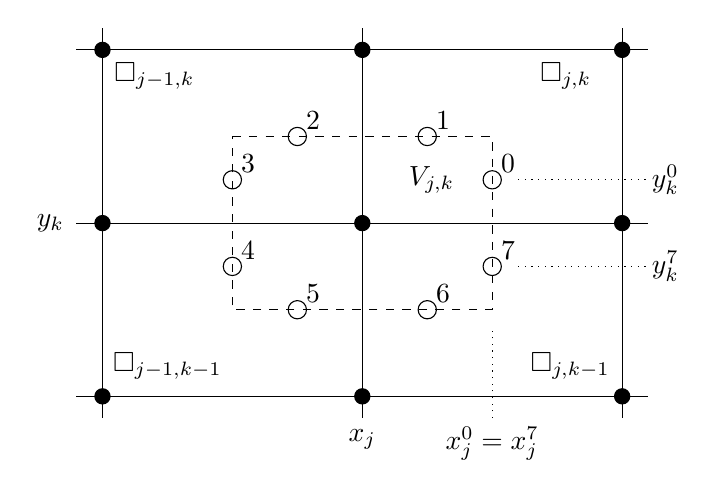
\begin{tikzpicture}[scale=1.1]
  %uncomment to see grid on which it was generated:
  %\draw[dotted,step=1.0,black,very thin] (0,0) grid (6,4);

  % strong grid around elements
  \draw (-0.3,0) -- (6.3,0);
  \draw (-0.3,2) -- (6.3,2);
  \draw (-0.3,4) -- (6.3,4);
  \draw (0,-0.25) -- (0,4.25);
  \draw (3,-0.25) -- (3,4.25);
  \draw (6,-0.25) -- (6,4.25);

  % nodes
  \filldraw (0,0) circle (2.5pt);
  \filldraw (3,0) circle (2.5pt);
  \filldraw (6,0) circle (2.5pt);
  \filldraw (0,2) circle (2.5pt);
  \filldraw (3,2) circle (2.5pt);
  \filldraw (6,2) circle (2.5pt);
  \filldraw (0,4) circle (2.5pt);
  \filldraw (3,4) circle (2.5pt);
  \filldraw (6,4) circle (2.5pt);

  % outline control volume
  \draw[dashed] (1.5,3) -- (4.5,3) -- (4.5,1) -- (1.5,1) -- cycle;

  % mark quadrature points

  \draw (4.5,2.5) circle (3.0pt) node[shift={(0.2,0.2)}] {0};
  \draw (3.75,3)  circle (3.0pt) node[shift={(0.2,0.2)}] {1};
  \draw (2.25,3)  circle (3.0pt) node[shift={(0.2,0.2)}] {2};
  \draw (1.5,2.5) circle (3.0pt) node[shift={(0.2,0.2)}] {3};
  \draw (1.5,1.5) circle (3.0pt) node[shift={(0.2,0.2)}] {4};
  \draw (2.25,1)  circle (3.0pt) node[shift={(0.2,0.2)}] {5};
  \draw (3.75,1)  circle (3.0pt) node[shift={(0.2,0.2)}] {6};
  \draw (4.5,1.5) circle (3.0pt) node[shift={(0.2,0.2)}] {7};

  % label elements and control volume
  \draw (3.8,2.5) node {$V_{j,k}$};
  \draw (5.35,3.7) node {$\square_{j,k}$};
  \draw (5.4,0.35) node {$\square_{j,k-1}$};
  \draw (0.6,3.7) node {$\square_{j-1,k}$};
  \draw (0.75,0.35) node {$\square_{j-1,k-1}$};

  % label center point
  \draw (3,-0.5) node {$x_j$};
  \draw (-0.6,2) node {$y_k$};

  % indicate coordinates of quadrature points
  \draw[dotted] (4.5,-0.25) -- (4.5, 0.8);
  \draw (4.5,-0.55) node {$x_j^0=x_j^7$};
  \draw[dotted] (4.8,2.5) -- (6.3, 2.5);
  \draw (6.5,2.5) node {$y_k^0$};
  \draw[dotted] (4.8,1.5) -- (6.3, 1.5);
  \draw (6.5,1.5) node {$y_k^7$};

\end{tikzpicture}

\end{center}
\caption{To compute the integral in equation \eqref{eq:siafve} more accurately, we evaluate $\bq^h(x,y)$ at eight quadrature points (circles) along $\partial V_{j,k}$, where $\bq^h$ is continuous.  The specific coordinates in equation \eqref{eq:starbreakfirst} are indicated.}
\label{fig:improvequadrature}
\end{figure}

Similar formulas to \eqref{eq:starbreakfirst} apply to the other three integrals on the right side of \eqref{eq:fluxintdecomp}.  Figure \ref{fig:improvequadrature} shows all eight quadrature points needed to compute the full integral over $\partial V_{j,k}$ in \eqref{eq:siafve}.  We see that the total number of flux-evaluation locations for the improved method is twice that for the classical method, but in fact the improved method evaluates $\bq^h(x,y)$ at only four locations \emph{in each element}, as does the classical Mahaffy method, which evaluates the flux at the midpoint of every side of every element.  The stencils for the two methods are the same.  That is, in both methods the discrete conservation equation---equation \eqref{eq:siasteadyfd} or \eqref{eq:siafve} according to interpretation---uses the same nine nodal values of $H^h$ (solid dots in Figures \ref{fig:fdfemgrids}a, \ref{fig:fdfemgrids}b, and \ref{fig:improvequadrature}).

Eight half-edges make up $\partial V_{j,k}$, with each half-edge entirely inside an element and $\bq^h$ smooth along each half-edge.  Thus one could propose further-improved methods, replacing the midpoint rule by higher-order quadrature (e.g.~2-point Gauss-Legendre quadrature).  Also, the $Q^1$ elements here could be replaced by higher-order $Q^2$ elements.  Though such methods have not been tested, we observe that the largest numerical SIA errors occur near the free boundary, namely at the ice sheet margin \citep{Bueleretal2005}.  At such locations the exact solution $H$ has low regularity \citep{JouvetBueler2012}.  Any FE method of any order therefore suffers in the sense that the exact free boundary may pass through an element.  Because $\bq^h$ represents a smooth approximation on the element to a merely-continuous (and not smooth) exact flux $\bq$, higher-order quadrature and interpolation will probably not give much advantage near the free boundary.  Our improved method represents a measurable improvement over the classical Mahaffy method (see the next section) primarily because the improved method evaluates the flux approximation $\bq^h$ at points of continuity, not because the midpoint rule or bilinear interpolation, both of which are implicitly used in the classical method, are flawed.

\cite{JaroschSchoofAnslow2013} show that the Mahaffy scheme suffers from significant mass conservation errors at locations of abrupt change in the bed elevation, even away from the free boundary.  (I.e.~even with positive thickness at all involved grid points.)  In such cases, when the bed gradient dominates the thickness gradient, the mass conservation equation has ``hyperbolic'' character.  They propose and demonstrate that a particular higher-resolution upwinding scheme \citep{LeVeque2002} based on the form $\bq = \boldsymbol{\omega} H^{n+2}$ of the entire SIA flux reduces error at such locations.  Their upwinding scheme expands the stencil of the scheme so that, for example, computing $\bq$ at point $(x_j,y_k)$ involves thickness $H_{j+2,k}$ which is two cells away.  Furthermore they use explicit time-stepping to update the thickness.  Compare to theirs, we propose an implicit (see next section), FE-based, stencil-non-expanding form of upwinding, but we use their bedrock-step exact solution for testing our scheme (see Examples section).  Note that for our implicit implementation, upwinding is not required for stability or non-oscillation in smooth bed cases.

First recall form \eqref{eq:fluxform}, which decomposes the flux into a diffusion term and a transport term.  We denote the transport term by $\tilde \bq$:
\begin{equation}
  \bq = - D \grad H + \tilde \bq \quad \text{where} \quad \tilde \bq = \bW H^{n+2}, \label{eq:transporttermdefine}
\end{equation}
and $\bW$ is computed by formula \eqref{eq:siaWdefine}.  So far we have evaluated the whole flux $\bq$ at each quadrature point, but we propose to upwind only the $\tilde \bq$ term, and only by changing the location where $H^{n+2}$ is evaluated.  Our evaluation of $D\grad H$ and $\bW$ are unchanged.

Recall that our improved scheme evaluates $\bq^h$ at quadrature point $(x_j^+,y_k+\tfrac{\Delta y}{4})$ shown in Figure \ref{fig:improvequadrature}, among other points.  We show the upwind modification at this point.  It uses the sign of the $x$-component $W^x$ of $\bW = (W^x,W^y)$ at the point, namely
\begin{equation}
W^x_* = W^x(x_j^+,y_k+\tfrac{\Delta y}{4}),
\end{equation}
to shift the evaluation of $H$ in $\tilde \bq$ upwind by a quarter of an element width:
\begin{align}
&\tilde \bq^x(x_j^+,y_k+\tfrac{\Delta y}{4})  \label{eq:upwindschemex} \\
&\quad = W^x_* \begin{cases}
                 H(x_j+\tfrac{\Delta x}{4},y_k+\tfrac{\Delta y}{4})^{n+2}, & W^x_* \ge 0, \\
                 H(x_j+\tfrac{3\Delta x}{4},y_k+\tfrac{\Delta y}{4})^{n+2}, & W^x_* < 0.
             \end{cases} \notag
\end{align}
Note that the sign of $W_x^*$ is fully-determined by---i.e.~opposite to---the sign of the $x$-component of the bed gradient $\grad b$; see equation \eqref{eq:siaWdefine}.

The upwind modification at this quadrature point is shown by horizontal arrows in Figure \ref{fig:upwindterm}.  Upwinding at the other seven points along $\partial V_{j,k}$ (Figure \ref{fig:improvequadrature}) is achieved by similar formulas.  Note that these upwinding modifications do not expand the stencil of the scheme \citep[compare][]{JaroschSchoofAnslow2013}.  Though this is a form of first-order upwinding in theory, the change is most important at locations of low regularity of the solution, and we will see in verification that it improves accuracy over the apparently second-order Mahaffy scheme.

\begin{figure}[ht]
\begin{center}
\begin{tikzpicture}[scale=1.8]
  %uncomment to see grid on which it was generated:
  %\draw[dotted,step=1.0,black,very thin] (0,0) grid (6,4);

  % strong grid around elements
  \draw (-0.3,0) -- (3.3,0);
  \draw (-0.3,2) -- (3.3,2);
  \draw (0,-0.3) -- (0,2.3);
  \draw (3,-0.3) -- (3,2.3);

  % nodes
  \filldraw (0,0) circle (1.5pt);
  \filldraw (3,0) circle (1.5pt);
  \filldraw (0,2) circle (1.5pt);
  \filldraw (3,2) circle (1.5pt);

  % outline control volume
  \draw[dashed, thick] (-0.25,1) -- (1.5,1) -- (1.5,-0.25);

  % mark quadrature points
  \draw (1.5,0.5)  circle (2.0pt);
  \draw (0.75,1.0) circle (2.0pt);

  % mark upwind points
  \draw (1.125,0.5) node {$+$};
  \draw (1.875,0.5) node {$+$};
  \draw (0.75,0.75) node {$+$};
  \draw (0.75,1.25) node {$+$};

  % arrows to suggest upwinding
  %\draw[-latex] (1.6,0.4) -- (1.80,0.4);
  %\draw[-latex] (1.4,0.4) -- (1.20,0.4);
  %\draw[-latex] (0.65,1.05) -- (0.65,1.2);
  %\draw[-latex] (0.65,0.95) -- (0.65,0.8);

  % label elements and control volume
  \draw (2.7,1.7) node {$\square_{j,k}$};

  % label lower-left corner
  \draw (0,-0.5) node {$x_j$};
  \draw (-0.5,0) node {$y_k$};

  % indicate coordinates of quadrature point
  \draw (1.5,-0.5) node {$x_j^0$};
  \draw[dotted] (2.8,0.5) -- (3.2, 0.5);
  \draw (3.4,0.52) node {$y_k^0$};

\end{tikzpicture}

\end{center}
\caption{On element $\square_{j,k}$, in computing the flux at quadrature points (circles), upwinding of the flux term $\tilde \bq = \bW H^{n+2}$ evaluates the thicknesses $H$ at locations shown with ``$+$'', according to the sign of the components of $\bW$.  These locations are along element diagonals (dotted).}
\label{fig:upwindterm}
\end{figure}

This upwind modification is the second of our two improvements over the classical Mahaffy scheme.  We call the method which combines these two improvements (quadrature and upwinding) the ``\Mstar'' method.  We will see that the primary benefit is in the convergence of the method for solving the system of nonlinear algebraic equations.  A secondary benefit is a small improvement in accuracy, especially on coarse grids.  In the Appendix we describe an unstructured-mesh version of the \Mstar scheme.


\section{Solution of the equations} \label{sec:solution}

We have, so far, proposed improvements to the local accuracy (i.e.~better quadrature) and stability with respect to bed elevation gradients (i.e.~upwinding) of the Mahaffy FD scheme, based on re-interpreting it as an FVE method.  The resulting \Mstar scheme allows us to assemble a system of nonlinear algebraic equations.  However, it remains to describe, at a high level appropriate to our advanced mathematical software tools, the numerical solution of the system.

We suppose that the structured grid covers a rectangular domain which has the easiest boundary conditions (b.c.s) appropriate to a whole ice sheet model, namely periodic b.c.s in both $x$- and $y$-directions.  For the Greenland computation in the next section the reader may suppose that these b.c.s are ``applied'' at locations in the deep ocean, but in fact ``periodic b.c.s'' simply means that all nodes see the same configuration of neighboring nodes.

If there are $N_x$ and $N_y$ nodes in each direction, respectively, then $N=N_x N_y$ is the number of total nodes, elements, and control volumes.  In \Mstar, each equation is simply equation \eqref{eq:siafve} with quadrature \eqref{eq:starbreakfirst} and upwind modification \eqref{eq:upwindschemex}, based on evaluating the everywhere-defined functions $H^h$ and $b^h$ in the FE function space $S_h$.  The resulting highly-nonlinear system of $N$ equations
\begin{equation}
F_{j,k}(\bH) = 0   \label{eq:nonlinsystem}
\end{equation}
relates $N$ unknowns $\{H_{j,k}\}$ which form a vector $\bH$.  Note $H^h$ and $\bH$ are two descriptions of the same discrete approximation to the thickness.

System \eqref{eq:nonlinsystem} is not, by itself, an adequate description because we must also respect $N$ inequalities
\begin{equation}
H_{j,k} \ge 0.  \label{eq:nonlinconstraints}
\end{equation}
Requirements \eqref{eq:nonlinsystem} and \eqref{eq:nonlinconstraints} can be combined into a variational inequality \citep{JouvetBueler2012,KinderlehrerStampacchia1980} or complementarity problem \citep{BensonMunson2006}.  In either formulation, we solve \eqref{eq:nonlinsystem} and \eqref{eq:nonlinconstraints} by a ``constrained'' Newton solver, specifically by the reduced-set method \citep{BensonMunson2006} implemented in PETSc \citep{Balayetal2014}.

The open-source C code used in the current paper\footnote{Clone the repository at \begin{center}\texttt{https://github.com/bueler/layer-conserve}\end{center}  Then see \texttt{README.md} in subdirectory \texttt{petsc/mahaffy/} to compile the code \texttt{mahaffy.c} and run the examples.  The residual-evaluating method in \texttt{mahaffy.c} is called \texttt{FormFunctionLocal()}.} is surprisingly brief because its only non-trivial part is a ``residual'' subroutine which records the equations \eqref{eq:nonlinsystem} themselves.  The Jacobian of system \eqref{eq:nonlinsystem}, i.e.~the $N\times N$ matrix
\begin{equation}
J = \left(\,\frac{\partial F_{j,k}}{\partial H_{r,s}}\,\right),
\end{equation}
is computed automatically and numerically within PETSc by finite-differencing \citep{Kelley2003}.  Numerical Jacobian evaluation is made efficient by ``coloring'' the nodes so that only nine evaluations of the residual are needed to compute the finite-difference derivatives \citep{CurtisPowellReid1974}, but, because of periodicity, the grid dimensions $N_x$ and $N_y$ must each be divisible by three.

A Newton solver requires an initial iterate $H^{(0)}$.  For this purpose we give a heuristic which seems to work adequately-well for both ice sheet and glacier scale problems.  From the steady surface mass balance data $m_{j,k}$, here measured in meters per year, we compute
\begin{equation}
H_{j,k}^{(0)} = \big(1000.0\,m_{j,k}\big)_+,  \label{eq:nonlininitialheuristic}
\end{equation}
where $x_+ = \max\{0,x\}$.  In other words, we build the initial iterate by simply piling up one thousand years of accumulation, without flow.

Additionally we apply a simple ``continuation'' scheme \citep[compare][]{KelleyKeyes1998} so as to start the Newton iteration with an easier problem, so as to work up to the fully nonlinear and degenerate SIA problem.  Consider this list of thirteen regularization values,
\begin{align}
\eps &= 1,\, 0.5,\, 0.2,\, 0.1,\, 0.05, \label{eq:continuationseq} \\
     &\qquad 0.02,\, 0.01,\, 0.005,\, 0.002,\, 0.001, \notag \\
     &\qquad 0.0005,\, 0.0002,\, 0, \notag
\end{align}
and define
\begin{align}
n(\eps) &= (1-\eps) n + \eps\, n_0,  \label{eq:continuationn} \\
D(\eps) &= (1-\eps) D + \eps D_0,  \label{eq:continuationD}
\end{align}
where $n$ is the original Glen exponent in \eqref{eq:siaflux}, $D$ is computed in \eqref{eq:siaflux}, $n_0=1$, and $D_0$ is a typical scale of diffusivities for the problem (e.g.~$D_0=0.1$ for a glacier problem or $D_0=10$ $\text{m}^2\,\text{s}^{-1}$ for an ice sheet).  Note $n(0)=n$ and $D(0)=D$.

We use \eqref{eq:continuationseq}--\eqref{eq:continuationD} as follows.  We solve \eqref{eq:nonlinsystem} and \eqref{eq:nonlinconstraints} with the first $\eps$ value from \eqref{eq:continuationseq}, thus with power $n(1)$ and diffusivity $D(1)$, using initial iterate $H^{(0)}$ from \eqref{eq:nonlininitialheuristic}.  Once the Newton solver for this problem converges, we take the solution as the initial iterate for problem \eqref{eq:nonlinsystem} and \eqref{eq:nonlinconstraints} but using the second $\eps$ value.  Continuing in this way we eventually solve the unregularized $n(0)=n$ and $D(0)=D$ problem.

Note that because $D(1)=D_0$, in the flat bed case the first of these continuation-method problems is actually a Laplacian obstacle problem \citep{KinderlehrerStampacchia1980}, namely $-\Div(D_0 \grad H) = m$ subject to the constraint $H\ge 0$.  Though this problem is nonlinear, because of the constraint which generates a non-trivial free-boundary problem, it is an easy problem on which the Newton solver can establish a first estimate of the ice-covered domain.

Now, before giving computed examples which justify our claim of practical, not just theoretical, stability, we should explain the relationship between our steady-state computations and fully-implicit time-stepping methods for the time dependent SIA evolution equation \eqref{eq:siaevolution}.  Our problem corresponds to taking infinite time steps in such a fully-implicit method.  Indeed, the backward-Euler \citep{MortonMayers2005} discretized form of equation \eqref{eq:siaevolution} is
\begin{equation}
\frac{H^\ell - H^{\ell-1}}{\Delta t} + \Div \bq^\ell = m \label{eq:backwardeuler}
\end{equation}
where $H^\ell(x,y) \approx H(t_\ell,x,y)$ is the unknown thickness, $H^{\ell-1}$ is known, and $\bq^\ell$ is the flux computed from \eqref{eq:siaflux} using $H^\ell$.  The constrained, continued, Newton, \Mstar method above extends easily to solving \eqref{eq:backwardeuler} at each time step.  For instance, the initial iterate can be taken to be the initial value or the result of solving at the previous time step, and the start of the continuation sequence can even be avoided.  If $\Delta t$ is not too big then actually \eqref{eq:backwardeuler} is also easier than the steady state limit $\Delta t\to \infty$, i.e.~equation \eqref{eq:siasteady}, because the Jacobian $J$ has a more-positive diagonal due to the $H^\ell/\Delta t$ term in \eqref{eq:backwardeuler}.  In fact, solving the steady state problem all at once is much harder than any single fully-implicit time-step.

\section{Examples} \label{sec:examples}

FIXME: verification on steady part of Test D from \cite{Bueleretal2005}, i.e.~``Bueler profile'' from \cite{vanderVeen2013}; at low res we see \Mstar is more accurate at points along margin; at high res \Mstar is slightly better for convergence

\begin{figure}[ht]
\onecol{domeprofile.pdf}
\caption{Result from \Mstar method on the Bueler profile exact solution ($\Delta x=25$ km).}
\label{fig:domeprofile}
\end{figure}

\begin{figure}[ht]
\onecol{domeverif.pdf}
\caption{Average and maximum error on the Bueler dome exact solution.}
\label{fig:domeverif}
\end{figure}

FIXME: verification on bedrock step solution from \cite{JaroschSchoofAnslow2013}

\begin{figure}[ht]
\onecol{bedstepprofile.pdf}
\caption{Result from \Mstar method on the Bueler profile exact solution ($\Delta x=500$ m).  The bed elevation is dashed.}
\label{fig:bedstepprofile}
\end{figure}

\begin{figure}[ht]
\onecol{bedstepverif.pdf}
\caption{Average and maximum error on the JSA bedrock-step exact solution.}
\label{fig:bedstepverif}
\end{figure}

FIXME: add whole Greenland model; compute \Mstar SIA solution with present-day climate in one step on fairly high res (1km); like \cite{JouvetBueler2012} result but much higher res and replacing fixed-point iteration by continuation 

FIXME: idea: because we solve implicitly, very little of high-res (e.g. TVD-diminishing) transport scheme theory carries over.  what is important, it appears, is the smoothness of the discrete approximation in the sense that a helpful Jacobian can be formed (whether fd or not, perhaps) that allows convergence at the $\eps=0$ (or near) level


\section{Discussion and Conclusion} \label{sec:conclusion}

FIXME: The first idea in the paper is that a FVE interpretation is compatible with the original Mahaffy FD scheme.  The second idea is that the flux approximation is discontinuous along element edges, so, in evaluating the quadrature along the boundary of the control volume, there is either a doubling of the range over which derivatives are evaluated (Mahaffy) or a doubling of the number of quadrature points (\Mstar).  The new \Mstar method is slightly more accurate, especially at coarse resolution, and easier to understand and implement in a $Q^1$ FE world.  The computed examples using this method are novel, except for \cite{JouvetBueler2012}, by going directly to steady state from zero ice.

\section*{Acknowledgements}
This work was supported by NASA grant \#NNX13AM16G and a grant of high-performance computing resources from the Arctic Region Supercomputing Center.


%         References
\bibliography{../layerpaper/lc}
\bibliographystyle{igs}

\appendix
\section{Appendix}  \label{sec:app}

FIXME: the same \Mstar idea can be extended to dual Delaunay/Voronoi meshes (e.g.~the meshes from \cite{EgholmNielsen2010,Ringleretal2013}) using $P^1$ elements on the Delaunay triangulation, and doing quadrature on the Voronoi-cell edges by splitting these edges where the element (i.e.~triangle) boundaries cross (perpendicularly) the Voronoi-cell edges.  This improves on the \cite{EgholmNielsen2010} method by exploiting an underlying $P^1$ element approximation to approximate the flux, instead of using the moving least squares method.


\begin{comment}
Here is what the MPAS Land-Ice User's Manual version 3.0 says:

\begin{quote}
\small
Velocities and fluxes are calculated on the midpoint of Voronoi cell edges.  The normal component of surface slope is calculated on cell edges using surface elevation at adjacent cell centers.  The tangential component of surface slope is calculated on cell edges using surface elevation at adjacent vertices. The surface elevation at vertices is calculated from the values at adjacent cell centers using barycentric interpolation. Ice thickness on edges is calculated as the average of the adjacent cell center values (2nd-order approximation).
\end{quote}

Looking at this, and the code, I don't think they think of it as Petrov-Galerkin
\end{comment}


\end{document}
